\documentclass[12pt,letterpaper]{article}
\usepackage{amsmath}
\usepackage[colorlinks]{hyperref} 
\usepackage[title,toc,page]{appendix}
\usepackage{graphicx}
\usepackage{caption}
\begin{document}

\title{Oh, What a Bot!}
\author{HackRVA.org}
\date{}
\maketitle



\section{Introduction}
This article describes the development of a control system model for an reaction wheel pendulum, shown in Figure \ref{sketchOfPendulum}.  A reaction wheel pendulum is a variation of a simple pendulum, balanced upright, with rotating wheels
at the top in place of the pendulum bob. Each wheel is driven by a separate motor.The pendulum is inherently unstable in the upright position - gravity will pull the pendulum over if it is not perfectly balanced.  Thus, a control system is needed to accelerate the reaction wheels, applying torques
as needed to the pendulum so as to keep it upright. The reaction wheels are mounted at right angles to each other, providing the ability to 
correct the alignment of the pendulum in any direction.

The pendulum physical structure includes a rod, an accelerometer, and two flywheels.  Each
flywheel is comprised of a motor mount, a DC brushed motor, and a reaction wheel.  The flywheel assemblies are mounted at
the top of the rod at right angles to each other and the rod.  The DC motors are wired to a motor controller and an Arduino.  The Arduino is also wired
to the accelerometer, which is located at the top of the rod.

\includegraphics[width=\textwidth]{images/pencil.png} 
    \captionof{figure}{Sketch of the Pendulum}  
    \label{sketchOfPendulum}





\section{Pendulum Dynamics}

Figure \ref{modelOfPendulum} shows a simplified sketch of the inverted pendulum.
Reference \cite{reactionWheel} contains a summary of the model dynamics for the balancing pencil.  
The model dynamics can be summarized as
%
\begin{equation}
    m g l \sin \theta - I_{c}\ddot{\theta}  = I_{f}\ddot{\phi}
\end{equation}
%
where: \\
$ m =$ total mass of inverted pendulum (kg)\\
$g =$ gravitational constant  (m s\textsuperscript{-2}) \\
$l =$ distance from the pivot point to the center of pendulum mass (m)\\
$\theta =$ pendulum angle (rad) \\
$I_{c} =$ moment of inertia of the pendulum (kg m\textsuperscript{2}) \\
$I_{f} =$ moment of inertia of the reaction wheel (kg m\textsuperscript{2}) \\
$\phi =$ flywheel angle (rad) \\

Other references may have alternate formulations using different definitions for $\theta$ and $\phi$.\footnote{Reference \cite{monograph} has a slightly different formulation for the model dynamics; 
the sign of the gravitational term is positive rather than negative.  This difference is caused 
by Reference \cite{monograph} defining the angle from the downward, resting position
while Reference \cite{reactionWheel} defines the angle from the vertical.  
The cosines of angles differing by $\pi$ have opposite signs.}\\


After linearizing the equation by noting that $\sin{\theta} \approx \theta$ for small angles, 
the transfer function for the pendulum is then
%
\begin{equation}
    m \,g \,l \theta - I_{c}\ddot{\theta}  = I_{f}\ddot{\phi}
\end{equation}
%
The reaction wheel can be continuously revolving, making the reaction wheel angle, $\phi$, less useful as a control parameter.
In its place we will use $\omega = \dot{\phi}$.
%
\begin{equation}
    m \,g \,l \theta - I_{c}\ddot{\theta}  = I_{f}\dot{\omega}\label{bigOne}
\end{equation}
%
For ease of use in later analysis, it is beneficial to split \eqref{bigOne} into two parts:
%
\begin{equation}
    m \,g \,l \theta + u(t)   = I_{c}\ddot{\theta}
\end{equation}
%
\begin{equation}
    u(t) = -I_{f}\dot{\omega}\label{oddOne}
\end{equation}
%
where $u(t)$ is the control torque applied to the pendulum.  The sign convention is important; a positive torque $u(t)$
will accelerate the pendulum in the direction of the positive pendulum angle.  However the sign convention in 
\eqref{oddOne} indicates that  a positive acceleration of the rotor will result in a \textit{negative} acceleration of the pendulum.

Note that if the pendulum is not vertical (i.e. $\theta = 0$) gravity will begin to pull the pendulum over.  Correcting this requires accelerating the flywheel to apply torque to the pendulum.  A flywheel turning at a constant velocity applies no torque to the pendulum and will not alter the movement of the pendulum.

Deriving the transfer functions,
%
\begin{equation}
    m \,g \,l \theta(s) + u(s) = I_{c}\theta(s) s^{2}
\end{equation}
%
\begin{equation}
    u(s)  = -I_{f}\omega(s) s
\end{equation}
%
\begin{equation}
    \frac{\theta(s)}{u(s)}= \frac{\frac{1}{I_{c}}}{s^{2} - \frac{m g l}{I_{c}} }
    \label{franco}
\end{equation}
%
\begin{equation}
    \frac{u(s)}{\omega(s)} = -I_{f} s
    \label{groucho}
\end{equation}\\


\includegraphics[width=\textwidth]{images/scan1.png}
    \captionof{figure}{Simplified Pendulum Model}
    \label{modelOfPendulum}






\section{Motor and Flywheel Dynamics}

Reference \cite{reactionWheel} models the motor as 
%
\begin{equation}
    I_{f} \, \ddot{\phi} \, \eta_{m} \, \eta_{g}  = K_{t} \, i
\end{equation}
%
where: \\
$\eta_{m} =$ motor efficiency \\
$\eta_{g} =$ gear efficiency \\
$K_{t} =$ motor torque constant (N m A\textsuperscript{-1}) \\
$i =$ motor current \\

This formulation appears to have problems, as a reduction in the motor and gear efficiencies results in a 
greater flywheel acceleration for a given motor current.  Similarly, the gear ratio above unity would 
decrease the flywheel acceleration for a specified motor current/torque, which is non-physical.  The equation can be altered
to correct these issues, resulting in the following:
%
\begin{equation}
	I_{f} \, \ddot{\phi} = \, \eta_{m} \, \eta_{g} K_{t} \, i
\end{equation}
%
However, this format may not be the easiest to implement, as the motor and gear efficiencies are not known.  Reference \cite{monograph}
takes a different approach,
%
\begin{equation}
    I_{f} \, \ddot{\phi} = T_{shaft}
\end{equation}
%
Where the earlier format dealt with motor/gear efficiencies using $\eta_{m}$ and $\eta_{g}$, Reference \cite{monograph} develops a correlation of friction in terms of torque required to maintain a given $\dot{\phi}$.  Here the torque will be
reformulated as 
%
\begin{equation}
    T_{shaft} = T - T_{friction}
\end{equation}
%
\begin{equation}
    T_{friction} = A \, sgn(\dot{\phi} ) + B \dot{\phi} 
\end{equation}
%
\begin{equation}
    T = K_{t} \, i
\end{equation}
%
where \\
$T =$ the total motor torque \\
$T_{shaft} =$ torque available to the flywheel \\
$T_{friction} =$ torque lost to motor and gear friction \\
$A =$ coulomb friction coefficient \\
$B =$ rotational friction coefficient \\

Combining equations and adding the reduction gear ratio,
%
\begin{equation}
    I_{f} \, \ddot{\phi}  = K_{t} \, i - A \, sgn(\dot{\phi} ) - B \dot{\phi}
\end{equation}
%
Again, using the notation $\omega = \dot{\phi}$,
%
\begin{equation}
    I_{f} \, \dot{\omega}  = K_{t} \, i - A \, sgn(\omega) - B \omega \label{wheel}
\end{equation}
%

As will be seen, this equation is easier to implement because $K_{t}$, $A$, and $B$ can be measured experimentally (see Appendixes \ref{appendix:measure} and \ref{appendix:friction}).







\section{Motor Control}
The previous chapter determined the relationship between the motor current and the acceleration of the flywheel.  
However, the motor will be not be controlled via motor current.  Instead, a motor controller will be used to control the 
motor by adjusting the motor voltage via a PWM signal.  The equivalent, average voltage will then regulate the motor.  
Reference \cite{monograph} give the relationship between motor current and voltage as
%
\begin{equation}
    L \, \frac{di}{dt} + R \,i = V - K_{v} \, \omega
\end{equation}
%
where: \\
$L =$ armature inductance (henry) \\
$R =$ armature resistance (ohm) \\
$V =$ voltage supplied to the motor (volt) \\
$K_{v} =$ motor voltage constant (V  rad\textsuperscript{-1} sec) \\
$\omega =$ motor rotation speed (rad sec\textsuperscript{-1}) \\

Normally the inductance of the motor is much lower than the resistance, such that $L/R \sim 0.001$.  
In such cases it is acceptable to ignore the time dependence of the current and write
%
\begin{equation}
    R \,i = V - K_{v} \, \omega \label{motor}
\end{equation}
%
Note that, provided mks units are used, $K_{v}$ and $K_{t}$ will have the same magnitude.  This can be seen by equating the 
mechanical and electrical power
%
\begin{equation}
    T \omega = V i
\end{equation}
%
where $T =$ is the motor torque.
Rearranging,
%
\begin{equation}
    \frac{T}{i} = \frac{V}{\omega}
\end{equation}
%
or
%
\begin{equation}
    K_{t} = K_{v} 
\end{equation}
%

Back to the motor equation, we can solve \eqref{motor} for i:
%
\begin{equation}
    i = \frac{V}{R} - \frac{K_{v} \, \omega}{R}
\end{equation}
%
Combining with \eqref{wheel}
%
\begin{equation}
    I_{f} \, \dot{\omega}  =  K_{t} \, \left( \frac{V}{R} - \frac{ K_{v} \, \omega}{R} \right) - A \, sgn(\omega ) - B \omega
\end{equation}
Rearranging,

\begin{equation}
    I_{f} \, \dot{\omega} + \left( B+\frac{K_{t} K_{v}}{R} \right) \omega +A \, sgn(\omega)= \left(\frac{K_{t}} {R}\right)V 
\end{equation}

Recognizing that $K_{t} = K_{v}$ and replacing them with $K$,
\begin{equation}
    I_{f} \, \dot{\omega} + \left( B+\frac{K^2}{R} \right) \omega +A \, sgn(\omega)= \left(\frac{K} {R}\right)V 
\end{equation}

Not all of the voltage results in acceleration of the reaction wheel.  As the reaction wheel velocity increases, an
increasing amount of the voltage (and the resulting torque) is consumed by friction and the back EMF.

We will assume that the control function can adjust the demand voltage by adding or subtracting a constant, depending on the current spin direction of the reaction wheel.  This means that $-A\,sgn(\dot{\phi})$ is folded
into $V$ for the purposes of this analysis.  The transfer function for the motor and flywheel is then:
\begin{equation}
    I_{f} \, \omega(s) s + \left( B+\frac{K^2}{R} \right) \omega(s) = \left(\frac{K} {R}\right)V(s)
\end{equation}
\begin{equation}
    \frac{\omega(s)}{V(s)} =  \frac{\left(\frac{K} {I_{f}R}\right)}{s + \frac{B R +K^2}{I_{f}R }}
    \label{rondo}
\end{equation} 
The characteristic equation for \eqref{rondo} is first order with a negative root, indicating that $\omega$ is controllable via $V$.








\section{Modeling in the Frequency Domain}
The primary objectives of a control system for the pendulum should be to stabilize the upright position of the pendulum and recovering from external forces on the pendulum.  In addition, the control system should be design to deal with a number
of physical limitations of the physical components of the pendulum.  Specifically,
\begin{itemize}
    \item the motor voltage is limited to maximum value,
    \item The rotor velocity has a practical upper limit.
\end{itemize}
The basic design of a control system for the pendulum is shown in Figure \ref{schematic}.  The pendulum is controlled
to a constant angle (r=0) intended to keep the pendulum vertical.  The Controller block can be used to implement a
form of feedback proportional to the error term.  $F$ represents a random environmental force that affects
the pendulum.  This sort of system design is often referred to as a Regulator Problem.  Analysis of this design may be more
clear if the schematic is rearranged as shown in Figure \ref{modifiedSchematic} to emphasize controlling $\theta$ in the presence of $F$.
\footnote{Note that in Figure \ref{schematic} the control signal and $f$ are added, while in Figure \ref{modifiedSchematic} the control signal is subtracted.  The "negative feedback" model in Figure \ref{modifiedSchematic} is achieved by noting that the rotor transfer function has a negative gain, 
resulting in a negative feedback.}\\

The stability of the system shown in Figure  \ref{modifiedSchematic} can be evaluated by examining the
open loop transfer function
\begin{equation}
    T(s) = P(s) C(s) M(s) R(s)
\end{equation}
where $P(s)$ is the pendulum transfer function \eqref{franco}, $C(s)$ is the control function, $M(s)$ is the motor transfer function \eqref{rondo}, and $R(s)$ is the rotor transfer function \eqref{groucho}.  
At this point in the analysis the control function will be assumed to be a unity gain.

Using \eqref{franco}, \eqref{groucho}, and \eqref{rondo} results in 
\begin{equation}
	T(s) =\frac{-(\frac{K} {I_{c}R})s}
	{s^3 + (\frac{BR+K^2}{I_{f}R})s^2 - (\frac{m g l}{I_{c}})s - (\frac{BR+K^2}{I_{f}R} - \frac{m g l}{I_{c}})}
\end{equation}

Substituting in values from the appendixes, the transfer function for the pendulum is
\begin{equation}
	T(s) =\frac{-0.2464 s}{s^3 + 4.7303 s^2 -34.8017 s -164.622}
\end{equation}

The numerator of the transfer function is the characteristic equation that, when factored, is
$(s-5.8993) (s+5.8993) (s+4.7303)$.

Using the root locus technique and the open loop transfer function, Figure \ref{rootLocus} shows the
behavior of the closed loop poles as a function of feedback gain.  Note that one pole is always in the right
half of the plane, indicating that the system is unstable regardless of the magnitude of the gain.

One possible method of stabilizing the system would be to use both proportional and derivative, or PD, feedback.  The control function would be.
\begin{equation}
	C(s) = 1 + r s
\end{equation}
Rearranging,
\begin{equation}
	C(s) = \frac{s+\frac{1}{r}}{r}
\end{equation}

indicating a zero at $1/r$ and a gain of $1/r$.
The results are sensitive to the placement of the zero.  Placing the zero to the right of the pole at -5.8993 
eliminates any oscilation, but does not remediate the pole in the right half of the plane.  Placing the zero to the left of the pole at -5.8993 results in a much faster response, but can result in oscillations (Figure \ref{rootLocusPD}).  Again, the pole in the right half of the plane is not remediated. \\


One possibility for resolving the issue of the zero at the origin would be to implement a PID controller.
\begin{equation}
	C(s) = 1 + \frac{r}{s} + q s
\end{equation}
Rearranging,
\begin{equation}
	C(s) = \frac{qs^2+s+r}{s}
\end{equation}

This controller would have two zeros that can be placed as required and a pole that would cancel
the zero at the origin.  If the zeros are placed to the left of the pole at -4.7303, then the system may stabilize.
However, in the real world the original zero may not be exactly at the origin and the poles in the left side of the axis may not be exactly where they are expected (due to nonlinearities, etc.) 
leading to a less-than robust control system. \\

Finally, it is possible to include feedback from the other monitored and controlled variable, the rotor velocity.
Unfortunately, to continue to evaluate the system using a root locus analysis, the feedback from
the rotor velocity will have to be directly factored into the transfer function.  \\

Here we modify \eqref{motor} to include the feedback from the rotor velocity:
\begin{equation}
    R \,i = V +K_{\omega}\omega - K_{v} \, \omega \label{motorUpdated}
\end{equation}

where: \\
$ K_{\omega} =$ rotor velocity feedback gain.\\

Solving for i,
\begin{equation}
    i = \frac{V}{R} - \frac{(K-K_{\omega}) \, \omega}{R}
\end{equation}

and

\begin{equation}
    \frac{\omega(s)}{V(s)} =  \frac{\left(\frac{K} {I_{f}R}\right)}{s + \frac{B R -K K_{\omega} +K^2}{I_{f}R }}
    \label{rondoMucho}
\end{equation} 

Using \eqref{franco}, \eqref{groucho}, and \eqref{rondoMucho}, the open loop transfer function is now
\begin{equation}
	T(s) =\frac{-(\frac{K} {I_{c}R})s}
	{s^3 + (\frac{BR-K K_{\omega}+K^2}{I_{f}R})s^2 - (\frac{m g l}{I_{c}})s - (\frac{BR-K K_{\omega}+K^2}{I_{f}R} - \frac{m g l}{I_{c}})}
\end{equation}

Figure \ref{rootLocusFull} shows the root locus with $r = 1/4.5$ and $K_{\omega} = 0.15$.  With a system gain of 510 the controlling poles are at -2.24 +/- 2.5i, a damping factor of 0.667, an overshoot of 6.01\%, and 
a frequency of 3.35 rad/second.

\includegraphics[width=\textwidth]{images/graph1.png} 
    \captionof{figure}{System Schematic with Controller}  
    \label{schematic}

\includegraphics[width=\textwidth]{images/graph2.png} 
    \captionof{figure}{Modified System Schematic with Controller}  
    \label{modifiedSchematic}

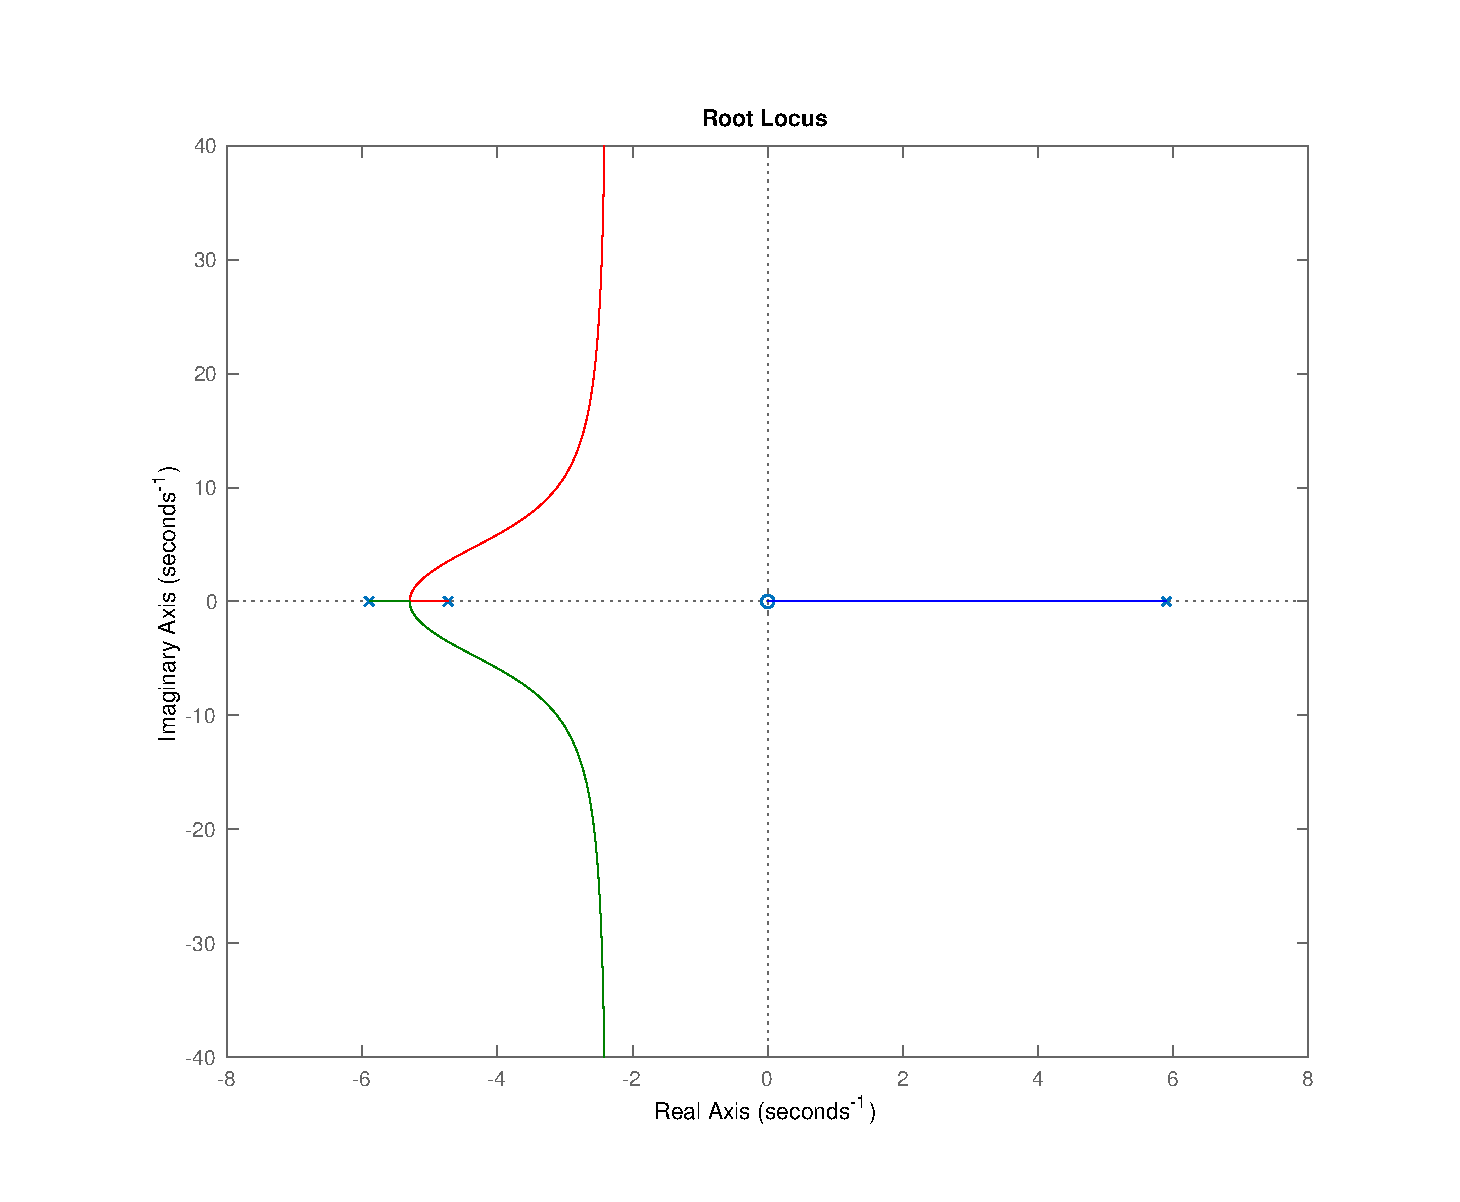
\includegraphics[width=\textwidth]{images/rootLocus.eps} 
    \captionof{figure}{Root Locus Plot With Proportional Feedback}  
    \label{rootLocus}

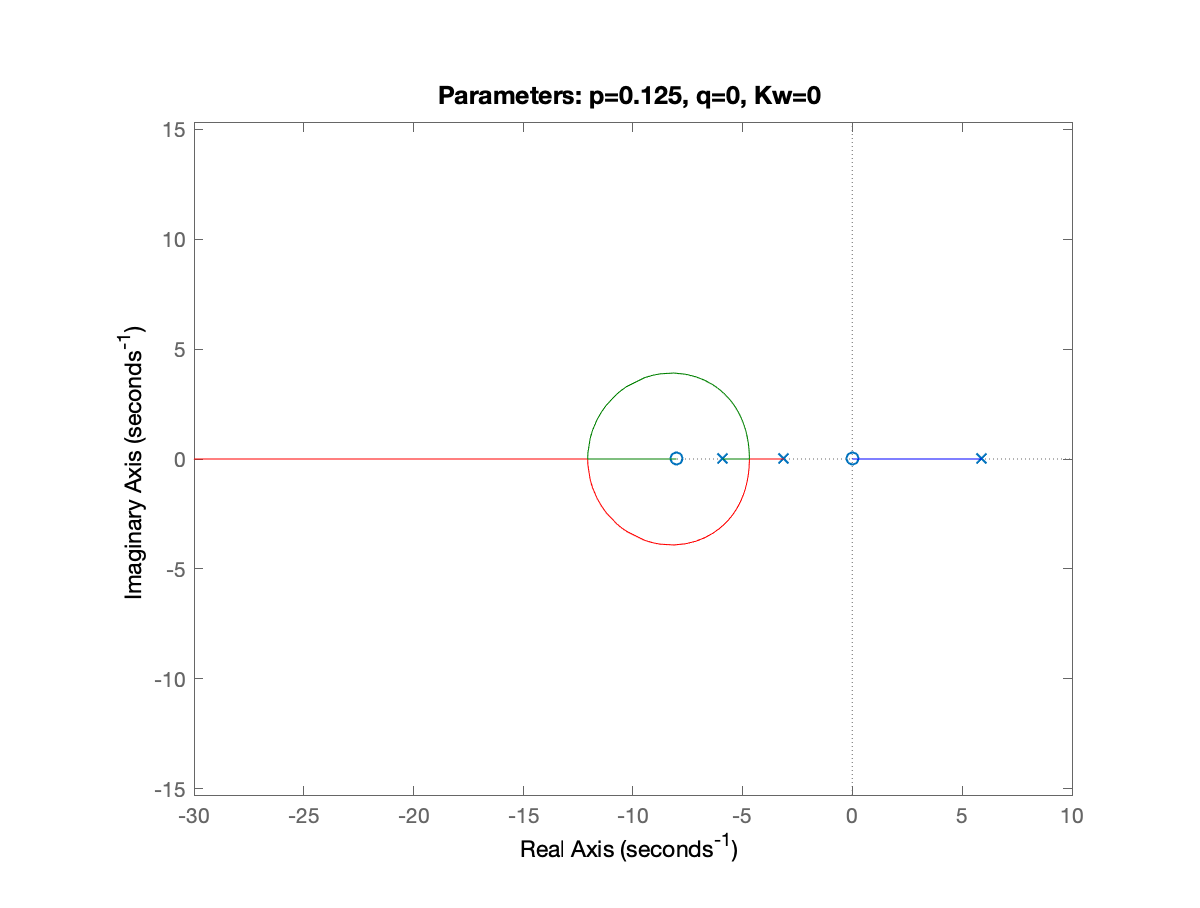
\includegraphics[width=\textwidth]{images/rootLocusPD.eps} 
    \captionof{figure}{Root Locus Plot With PD Feedback}  
    \label{rootLocusPD}

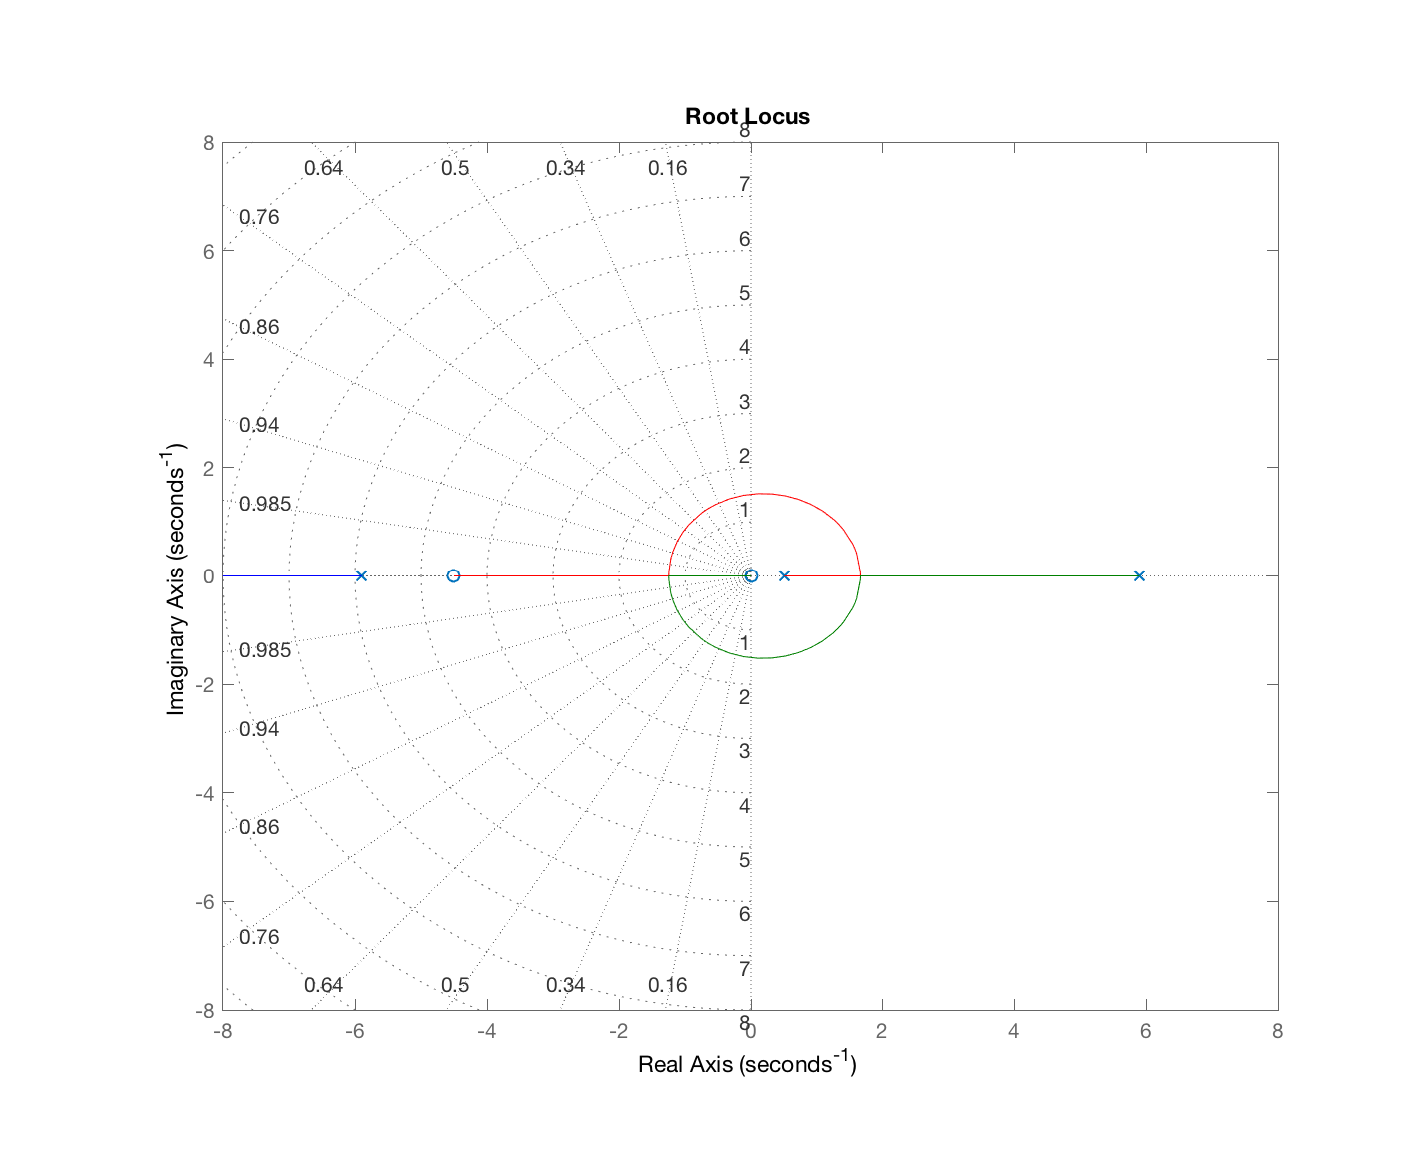
\includegraphics[width=\textwidth]{images/rootLocusFull.eps} 
    \captionof{figure}{Root Locus Plot With PD and Rotor Velocity Feedback}  
    \label{rootLocusFull}









 
\begin{thebibliography}{99}
\bibitem{monograph} Block, D. J., Astrom, K. J., and Spong, M. W. (2007).  \emph{The Reaction Wheel Pendulum} . Morgan \& Claypool Publishers.
\bibitem{reactionWheel} \href{http://www.diva-portal.se/smash/get/diva2:916271/FULLTEXT01.pdf}{Ramm, A., and Sjostedt, M. (2015). Reaction wheel balanced robot, Design and Sensor Analysis of Inverted Pendulum Robot. Technical Report, KTH Royal Institute of Technology.}
\bibitem{balanceBot} \href{https://kth.diva-portal.org/smash/get/diva2:916184/FULLTEXT01.pdf}{Hellman, H. and Sunnerman, H, (2015).  Two-Wheeled Self-Balancing Robot. Technical report, KTH Royal Institute of Technology.}
\bibitem{twoWheeled} \href{http://geoffrey.chauveau.free.fr/pendulum/reports/final_report.pdf}{Chauveau, G., Chazal, D., Nakayama, D., Olsen, E., and Palm, S., (2005).  Controlling the Reaction Wheel Pendulum.}
\end{thebibliography}

\begin{appendices}

\section{Motor and Gear Set Data}

Key to much of the work so far are the constants associated with the motor and gear set, $K_{t}$, $K_{v}$, $R$, and $L$.
Here we are using a \href{https://www.pololu.com/product/3237}{Pololu  4.4:1 metal gear motor}.  

Pololu gives the following parameters for the 4.4:1 gear motor: \\
weight = 95g \\
gear ratio = 4.4:1 \\
No-load speed @ 12V = 1700 rpm (178 rad/sec)\\
No-load current @ 12V = 0.2 A \\
Stall current @ 12V = 2.1 A \\
Stall torque @ 12V = 11 oz in (0.07768 Nm)\\
Encoder frequency = 211.2 counts/rev of gearbox shaft\\

A number of the motor constants can be calculated from the published Pololu parameters.  However, it
should  be noted that, for inexpensive motors, the actual motor parameters may vary from the 
published data.  In any event, the motor constants will be calculated here and then later compared
with measured data.

$K_{f}$ can be calculated directly from the stall current, gear ratio, and torque: $K_{f}$ = 0.07768 Nm /  2.1 A = 
0.0370 Nm/A.  $K_{v}$ can be set equal to $K_{f}$, or 0.0370 Vs.

The motor winding resistance can be determined from the rated voltage and the stall current, as no back-EMF is occurring at stall
conditions.  Thus, $R$ = 12 V / 2.1 A = 5.7 ohms.



\section{Pendulum Constants}
A multitude of other values were calculated in MATLAB.  \\

\begin{tabular}{l l}
$m$ & 0.517327 kg \\
$l$ & 0.319038 m \\
$I_{c}$ & 0.046508 kg m\textsuperscript{2} \\
$I_{f}$ & 0.000164 kg m\textsuperscript{2} \\
$g$ & 9.81 m s\textsuperscript{-2} \\
\end{tabular}




\section{Measuring Motor Constants}
\label{appendix:measure}
Measurements were made to determine a number of motor constants, including $R$, $L$, and $K_{v}$.  

$R$ was measured using an EXTEC LCR meter, on the $R_{DC}$ setting, as 5.82 $\Omega$. $L$ was 
measured with the same instrument as 5.994 mH at 1kHz.  This gives a motor electrical time constant $L/R$ of 0.001 sec.  This is the time taken by the current in the motor to go from rest to 63\% of the final steady-state current.

$K_{v}$ was measured by driving a motors with a constant voltage and
varying loads while measuring $V$, $i$, and $\omega$.  


The motor was driven with a 12 V power supply.  The current was measured by the power supply.  Measuring current in this manner can have larger uncertainties, but comparing with measurements from a $\mu$Current DVM adapter indicated that the power supply current measurement was reasonable.  


$\omega$ was measured using the motor's encoder and an Arduino.  The encoder measured the shaft speed, not the gear-set speed.  However, a conversion coefficient of 211.2 counts/revolution was used to convert the encoder pulse rate to gear set rotation speed.

The following table shows the results for three different loads.  The first load was just rotor friction.  The second load added the Pololu hub adapter.  The third load included a plastic wheel attached to a propeller to increase the drag.
The resulting measured values are as follows: \\

\begin{tabular}{|c|c|c|c|c|c|}
\hline
Case & $v$ & $i$ & speed & $\omega$ & $\omega$ \\
      & (volts) &  (A) & (counts/sec) & (RPM) & (sec\textsuperscript{-1}) \\
\hline
1    & 11.95 & 0.0675 & 5,942.2   & 1,688.1   & 176.74 \\
2    & 11.95 & 0.075   & 5,923.58 & 1,682.83 & 176.19 \\ 
3    & 11.95 & 0.153   & 5,574.88 & 1583.77  & 165.82 \\
\hline
\end{tabular}

Calculating $K_{v}$ can be approached two ways.  The first is to solve \eqref{motor} using the measured
value of $R$.  The resulting values of $K_{v}$, one for each case, are:

\begin{tabular}{|c|c|}
\hline
Case & $K_{v}$  \\
         & (V sec) \\
\hline
1    & 0.0654  \\
2    & 0.0653  \\
3    & 0.0667  \\
\hline
\end{tabular}

A second approach is to use two cases in \eqref{motor} and solve simultaneously for $R$ and $K_{v}$.
Cases 1 and 3 were chosen because of the largest difference in $i$, attempting to ensure that the two
cases are independent.  This results in a values of $R$ = 8.24 $\Omega$ and $K_{v}$ = 0.0645 V sec.

The value of $K_{v}$ is fairly consistent with the values determined in the first approach, but the value
of $R$ appears to be high.  This may be caused by the limited change in $i$ in the data.  Use of a larger
load torque might result in a larger value of $i$ and a better estimate of $R$.  However, for the purposes
of this work the following values will be used:

\begin{tabular}{|c|c|c|}
\hline
R                   & $K_{v}$  & $K_{t}$ \\
($\Omega$)   & (V sec)   & (N m A) \\
\hline
5.82    & 0.0667  & 0.0667  \\
\hline
\end{tabular}

\section{Measuring Motor Friction Constants}
\label{appendix:friction}
Friction in the motor was evaluated by measuring the supply current as a function of motor speed.
The friction force is related to the motor current as $F = K_{t} i$.  The measurement was performed
by using a power supply with a variable current limit.  For various currents the speed of the motor
was measured by monitoring the motor encoder output with an Arduino.  The current was measured
both at the power supply as well as with a $\mu$Current DVM adapter.

The following data was collected:

\begin{tabular}{|c|c|c|c|c|c|}
Supply Voltage & Supply Current & $\mu$Current & Speed & Speed & Speed\\
(volts) & (amps) & (A) & (pulse/sec) & (rpm) & radians/sec\\
\hline
10.90 & 0.068 & 0.0676 & 5417 & 1538.9 & 161.16\\
10.04 & 0.063 & 0.0627 & 5001 & 1420.7 & 148.78\\
9.09 & 0.058 & 0.0596 & 4520 & 1284.1 & 134.47\\
7.93 & 0.056 & 0.0562 & 3937 & 1118.5 & 117.13\\
6.99 & 0.055 & 0.0550 & 3465 & 984.4 & 103.08\\
6.00 & 0.051 & 0.0521 & 2953 & 838.9 & 87.85\\
5.00 & 0.047 & 0.0500 & 2437 & 692.3 & 72.50\\
4.04 & 0.046 & 0.0483 & 1960 & 556.8 & 58.31\\
3.57 & 0.046 & 0.0486 & 1701 & 483.2 & 50.60\\
3.02 & 0.047 & 0.0481 & 1421 & 403.7 & 42.27\\
2.52 & 0.045 & 0.0459 & 1169 & 332.1 & 34.78\\
2.02 & 0.042 & 0.0437 & 910 & 258.5 & 27.07\\
1.51 & 0.039 & 0.0409 & 662 & 188.1 & 19.69\\
1.02 & 0.034 & 0.0366 & 414 & 117.6 & 12.32\\
0.47 & 0.031 & 0.0328 & 148 & 42.0 & 4.40\\
\end{tabular}

The encoder speed, in pulses/sec, was converted to RPM using the encoder frequency of 211.2
counts/revolution.

The Excel regression function was used to fit the $\mu$Current current measurement as a function
of the speed in radians/sec.  The regression intercept represents the fixed Coulomb friction and the
slope represents the viscous friction.  The regression results were 2.47E-3 N m and 1.20E-5 N m/(radian/sec),
after converting from current using $K_{t}$.  The coulomb friction represents approximately 3\% of the 
motor stall torque.  At the motor's no-load speed the viscous friction would double the total friction to 
approximately 6\% of the motor stall torque.  The viscous friction coefficient is significantly larger than
the value of 9.06E-7 N m/(radian/sec) measured in Reference \cite{twoWheeled}.  This may be due to
the gearbox associated with the motor used in the current work.  In any event, the friction will be included
in the system modeling.


\section{Arduino Code for Measuring RPM}




\end{appendices}


\end{document}
